\documentclass[12pt]{article}
\usepackage{fullpage,graphicx,psfrag,amsmath,amsfonts,verbatim}
\usepackage[small,bf]{caption}
\usepackage[hidelinks]{hyperref}
\usepackage{color}
\usepackage{minted}
\usepackage{subcaption}
\usepackage{pgfplots}
\usepackage{amsmath}
\usepackage{tikz,psfrag}

\input defs.tex

\bibliographystyle{alpha}

\title{QuantFy: Predictive Market Behavior App using Machine Learning }
\author{Balagangadhar Bathula}

\begin{document}
\maketitle

\begin{abstract}
Investment firms, hedge funds and even individuals have been using financial models to better understand market behavior and make profitable investments and trades.  To maximize return of investment these firms use large amounts of historical data and apply machine learning algorithms to the process.
QuantFy is an application (app) that would build predictive/optimized models using machine learning models such as linear regression, random forests and $k$-nearest neighbour. 


\end{abstract}

\newpage
\tableofcontents
\newpage
\listoffigures
\newpage
\listoftables
\newpage

This is description document for the Capstone project for Machine Learning Nanodegree program of Udacity. 

\section{Domain Background}
\label{sec:background}
Many financial, high frequency trading (HFT), and hedge fund companies are analyzing trading strategeis including algorithmic steps from information gathering to market orders using machine-learning approaches. This project proposes to apply these probabilistic techniques to make trading decisions. Using approaches such as linear regression, Q-learning, $k$-NN and regression trees and apply them to the actual trading situations.

This application software will be build using Python tools \cite{PyFi}. The book \cite{HeFu} provides a comprehensive overview of domain knowledge that would be required to understand the financial market world. Also the speicifications given \cite{GeTechCourse} will be used as guidelines to build this application. 

\section{Problem Statement}
\label{sec:prob}
Using the historical data for prices and performance statistics as features, we can get predicted future price of the stock. For instance we can set of performance statistics (such as Bollinger bands,  price-to-earning (P/E) ratio) as features of the present date mapped to price (say one week forecast which is an input) of price.
This creates a data set $<X,Y>$, where $X$ is the set of features and $Y$ as trading days.  Features used are the measurable quantities that a particular stock could use in the predicting things such as change in price, market relative change in price or simply future stock price. Few questions that one would ask, before getting started are-
\begin{enumerate}
\item Breath and depth of data: How much historical data one would like to consider?
\item What ticker symbols are you going to use?
\end{enumerate}
General machine learning models that can be used for this problem are:
\begin{enumerate}
\item Regression
\item $k$-nearest neighbors
\item Random Forests
\item Time-series analysis: This analysis will be used to estimate the commodity prices such as oil/gas etc. For instance we can observe long term trend in the time-series (such as exponential) and fit an exponential model to predict the future price. Using the concepts of \underline{drift} and \underline{seasonality}, build models for commodity stocks.
\end{enumerate}

\section{Project Design}
\label{sec:design}


Design phase of the QuantFy application consists of following phases:
\begin{itemize}
\item Time-series plots for the various stocks can be visualized at this link: \href{http://quantfy.herokuapp.com/price_plot}{\color{blue}{Price plot}} \cite{pp}. This link also computes various other technical indicators such as the SMA, Bollinger bands, etc.
\item Portfolio optimizer: Analyzing using stock price data, and using numerical optimization techniques, this has already been implemented in the app. Link to the app is \href{http://quantfy.herokuapp.com/portfolio}{\color{blue}{\bf Portfolio optimizer}} \cite{po}

\item Investment and Trading using machine learning: This was be built using the machine-learning stratagies such as (1) $k$-nearest neighbors (2) Random forests (3) Linear regression  and (4) Ridge regression. One can compare the performance of any two algorithms in the application. For more details, visit the application at \href{http://quantfy.herokuapp.com/mlModels}{\color{blue}{\bf ML models}}

\subsection{Software}
\begin{enumerate}
\item Front-end: Python \texttt{flask} based web application
\item Back-end: Python libraries, such as \texttt{scikit-learn, pandas, numpy, scipy, bokeh}.
\item Hosting platform: Heroku
\end{enumerate}

This  application can be accessed at: \href{http://quantfy.herokuapp.com}{\color{blue}{\bf QuantFy}} \cite{qfy}. The current version of the source code for this application can be found at this GitHub link: \href{https://github.com/beegeesquare/QuantFy}{\color{blue}{\bf Source code}} \cite{sc}

\section{Datasets and Inputs} 
\label{sec:datasets}
There are many open APIs to extract data:
\begin{enumerate}
\item Yahoo Finance:
\begin{enumerate}
\item Using an API call  \texttt{http://ichart.finance.yahoo.com/table.csv?s=\{YOUR\_SYMBOL\} }we can query and get historical data.
\item We can also use \texttt{yahoo\_finance} python library or,
\item We can also use \texttt{pandas\_datareader}
\end{enumerate}
\item Quandl: Using \texttt{quandl} python API we can get the historical data
\item Bloomberg API
\end{enumerate}
Current version of QuantFy application proposes to uses Quandl to get historical data and Yahoo Finance source will be added in the subsequent versions. One can extract more than 10 years of historical stock prices for many ticker symbols. 

\begin{figure}[!htbp]
\begin{center}
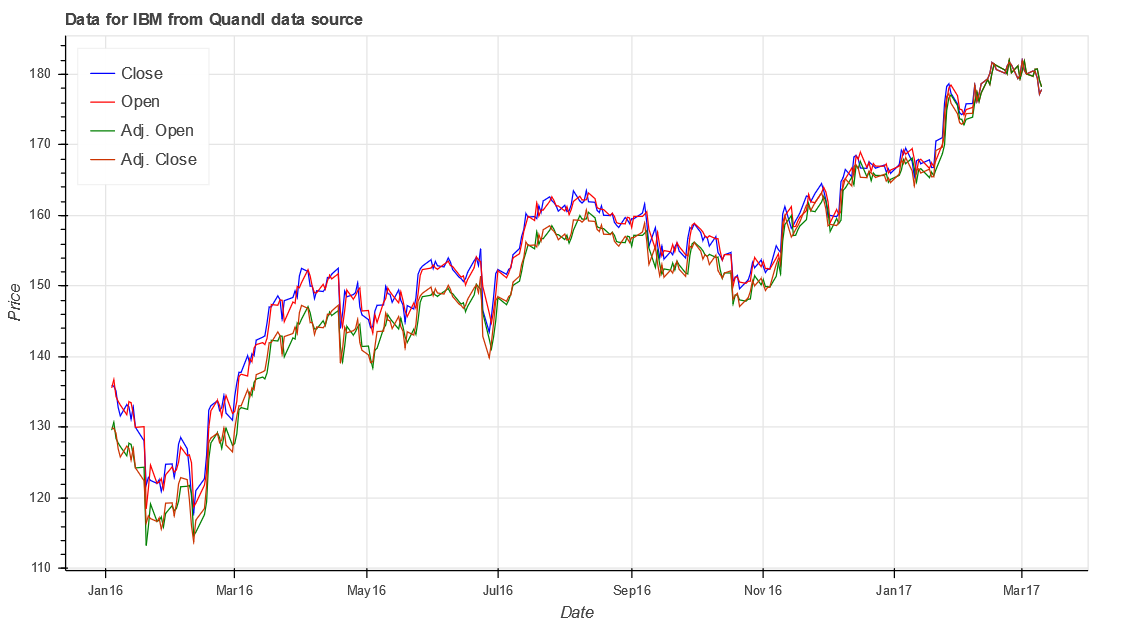
\includegraphics[height=0.5\textheight,width=\textwidth]{price_plot_IBM.png}
\caption{IBM prices from Jan 1 2016, from Quandl data source}
\label{fig:ibm_price}
\end{center}
\end{figure}

For instance user can specify the date range for viewing the stock prices of ticker symbols. Then an request call will be made and acquired data will be converted into a \texttt{pandas}  dataframe. This data will also be stored locally, using python libraries such as \texttt{ediblepickle}, so when the same request is made (no change in the parameters), data is retrieved locally. Since the data is generated online (rather than locally available data), we are not particularly concerned about the storing the data. At least from the past experience, the stock price data can be easily stored in the dataframe without any memory errors. We anticipate that the historical prices for the each ticker symbol will be in the order of less than 1 MB.

\begin{enumerate}
\item Close price and/or Adjusted close price
\item Start price and/or Adjusted start price,
\item Opening price  and/or adjusted opening price
\end{enumerate}

The data from these sources consists of features like:


\begin{figure}[!htbp]
\begin{center}
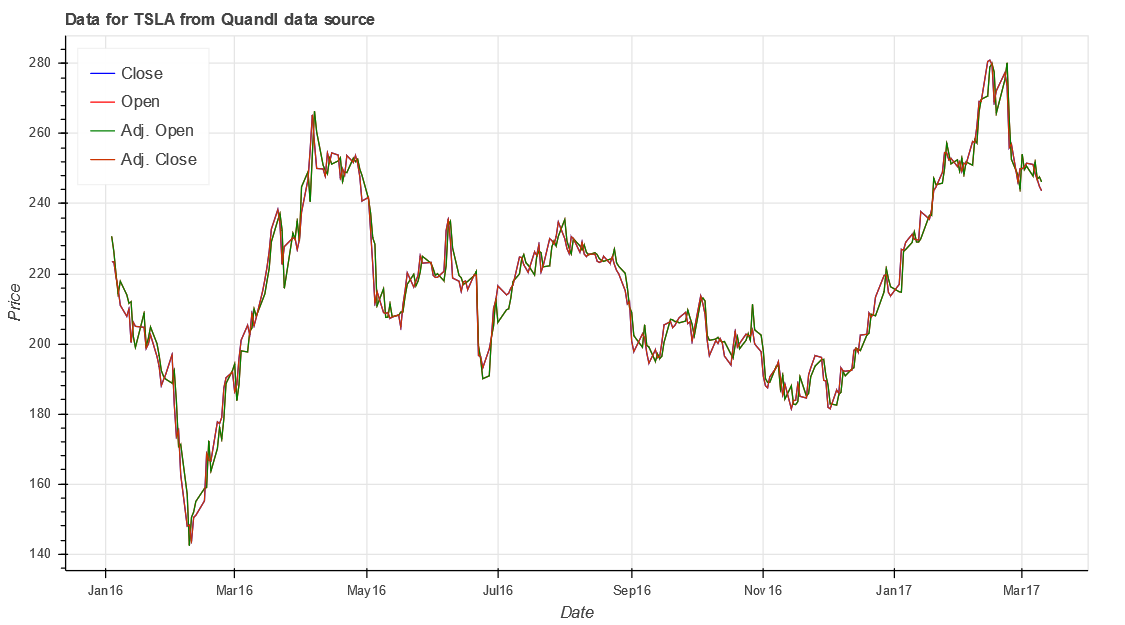
\includegraphics[height=0.5\textheight,width=\textwidth]{price_plot_TSLA.png}
\caption{Tesla prices from Jan 1 2016, Quandl data source}
\label{fig:tsla}
\end{center}
\end{figure}

\begin{figure}[!htbp]
\begin{center}
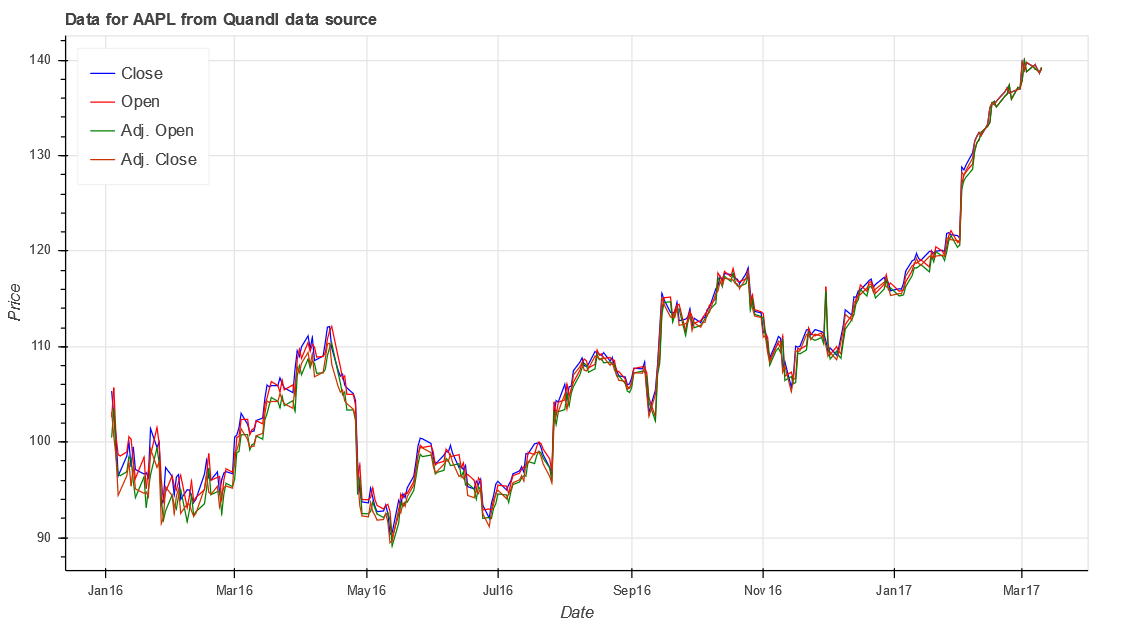
\includegraphics[height=0.5\textheight,width=\textwidth]{price_plot_AAPL.png}
\caption{Apple prices from Jan 1 2016, Quandl data source}
\label{fig:aapl}
\end{center}
\end{figure}

Snapshot of the plot prices for IBM, TSLA (Tesla) and AAPL (Apple) are shown in Figure~\ref{fig:ibm_price}, \ref{fig:tsla}, and \ref{fig:aapl} respectively. For more detailed refer to the application website \href{http://quantfy.herokuapp.com}{\color{blue}{\bf QuantFy}} \cite{qfy}. Table~\ref{tab:params}, describe the parameters for the data, such as count, mean, standard deviation etc. This can is achieved using the \texttt{describe()} option in pandas.

\begin{table}
\begin{center}
\begin{tabular} {|c|c|c|c|}
\hline \hline
\textbf{Metric} & \textbf{IBM} & \textbf{TSLA} & \textbf{AAPL} \\ \hline
Count & 300 & 300 & 300 \\ \hline
Mean & 151.4008 & 216.3058 & 107.5923\\ \hline
Standard deviation   & 15.7737 & 25.3987&12.2136  \\ \hline
Minimum & 113.8011 & 143.67 & 89.47 \\ \hline
25\% percentile & 143.5718 & 199 & 96.9126 \\ \hline
50\% percentile  & 151.7834 & 215.205 & 107.1624\\ \hline
75\% percentile  & 151.7834 & 215.205 & 107.1624 \\ \hline
Maximum  &  151.7834 & 215.205 & 107.1624\\ \hline
\hline
\end{tabular}
\end{center}
\caption{Description of the data for the stock symbols IBM, TSLA, AAPL}
\label{tab:params}
\end{table}

\section{Analyzing the stock price data}
\label{sec:anal}

When getting the stock price data for the ticker symbols, one need to clean the data to see if there are any un-available data points. For instance the stock has not traded a day, then it is mostly likely the exchange is closed. These \texttt{NaN} values have to be removed from the data-set. The most common way to do it this is to align the ticker symbol with the a benchmark symbol, say S\&P500 company and drop any \texttt{NaN} values in the data set. Also, we drop dates at which the S\&P500 has not traded. Sometimes the company's stock price might not be available, as it did not have an IPO (initial public offering) for the date. So we need to remove such data points as well. For example if we get the stock price of the \texttt{GOOG} from year 2010, then there will be \texttt{NaN} until year 2014. In \texttt{pandas} we can accomplish this with \texttt{df=df.dropna(axis=0)}, where \texttt{df} is the dataframe, and \texttt{dropna()} drops any values with \texttt{NaN} along the rows (\texttt{axis=0}).






We use adjusted close price is what we use for the rest of the discussion. Along with these features, one could compute other features like:

\begin{enumerate}
 \item \underline{Daily returns (DR)}: How much the price will go up or down on a particular instance of time:
 \begin{equation}
 \label{eq:dr}
r(t)=\frac{p(t)}{p(t-1)}-1,
\end{equation}

where $p(t)$ is the price at time $t$.

\item \underline{Average daily return (ADR)}: This is simply the average value of the the daily returns.
\begin{equation}
 \label{eq:adr}
  adr = \frac{\Sigma_{t=1}^{N} r(t)}{N}
\end{equation}

\item \underline {Cumulative daily return (CDR)}: Defined as the ratio of the final value of the the daily return to the initial value of the daily return 
\begin{equation}
 \label{eq:cdr}
cdr= \frac{r(N)}{r(0)},
\end{equation} 
where $N$ is the last sample point in the series.

\item \underline {Standard deviation of DR}: It is simply the standard deviation of the daily return ($r(t)$), which is the square-root of the variance.

\item\underline{Cumulative return} is given by,

\begin{equation}
 \label{eq:cr}
 cr(t)=\frac{p(t)}{p(0)}-1
\end{equation}

\item \underline{Simple moving average (SMA)}: Also know as moving average
  {\small \begin{minted}{python}
rolling_df=pd.DataFrame(index=df.index)
rolling_df =pd.Series.rolling(df,window=window).mean().to_frame() 
rolling_df.ix[:window, :] = 0
 \end{minted}
}

Table 2 shows the computed parameters for the data. Also, the other parameters are plotted in Fig. 4, 5 and 6 respectively.
\begin{table}
\begin{center}
\begin{tabular} {|c|c|c|c|}
\hline \hline
\textbf{Metric} & \textbf{IBM} & \textbf{TSLA} & \textbf{AAPL} \\ \hline
Cummulative daily return & 0.368 & 0.091 & 0.348 \\ \hline
Average daily return & 0.0011 & 0.00056 & 0.0011\\ \hline
Standard deviation of daily return  & 0.012 & 0.023 & 0.014  \\ \hline
Sharpe ratio & 1.49 & 0.38 & 1.23 \\ \hline
\hline
\end{tabular}
\end{center}
\caption{Parameters computed for the stock symbols IBM, TSLA, AAPL}
\end{table}

\begin{figure}[!htbp]
\begin{center}
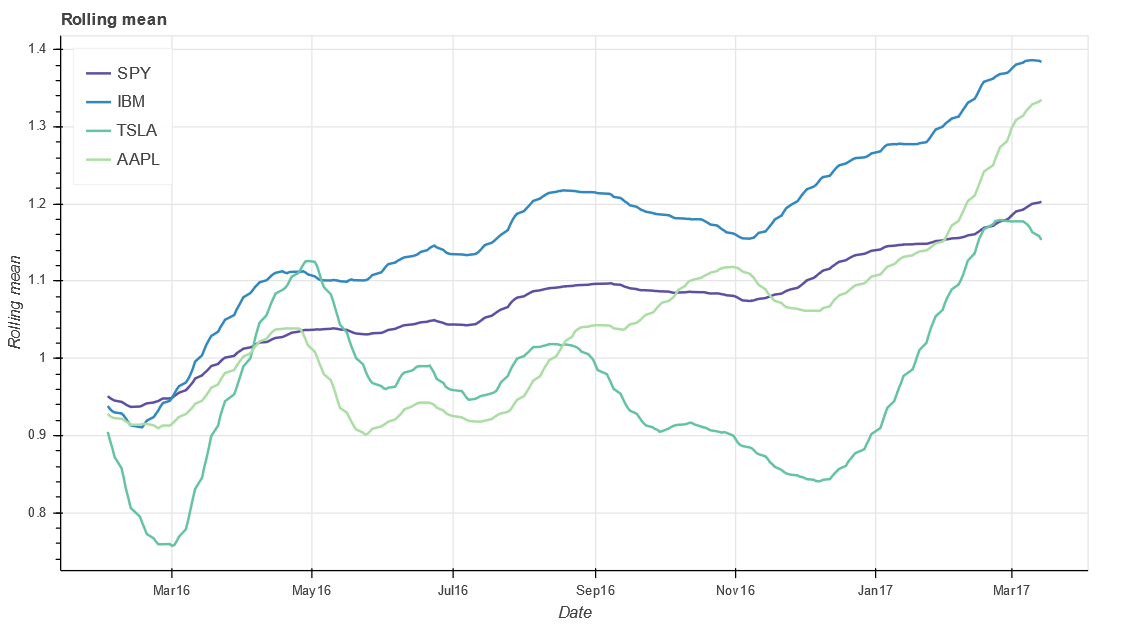
\includegraphics[height=0.4\textheight,width=\textwidth]{rolling_mean.png}
\caption{Rolling mean for the symbols IBM, TSLA and AAPL}
\label{fig:rm}
\end{center}
\end{figure}

\item \underline{Bollinger bands}: 

\begin{eqnarray}
\label{eq:bb}
 U_{band}& = & m_r+2\times\sigma_r, \nonumber \\
L_{band}& = &m_r-2\times\sigma_r
\end{eqnarray}

where $m_r$ is the rolling mean and $\sigma_r$ is the rolling standard-deviation of the adjusted close price.

\item \underline{Normalized Bollinger bands}: Value varies between -1.0 and 1.0.

\begin{equation}
 \label{eq:bb_norm}
 bb_{norm}=\frac{price[t]-SMA[t]}{2\times\sigma[t]}
 \end{equation}

where $\sigma$ is the rolling standard deviation and $SMA$ is the simple moving average. 

\item \underline{Sharpe ratio} This metric adjusts the return for risk, also know as risk adjusted reward.
\begin{equation}
 \label{eq:sr}
	sr= \frac{R_p-R_f}{\sigma_p},
\end{equation}

where $R_p$ is the portfolio return, $R_f$ is risk-free return and $\sigma_p$ is the standard deviation of portfolio return. 
\begin{equation}
 \label{eq:sr}
 sr=\frac{E[R_p-R_f]}{\sigma[R_p-R_f]}
 \end{equation}
 
Sharpe ratio varies depending on how frequently you sample the data. $sr_f=k\times sr$, where $k=\sqrt{\mbox{\# samples/year}}$

\item \underline{Volatility} is nothing but the standard deviation of the daily returns.

\begin{equation}
 \label{eq:vol}
 v(t)=\sqrt{var[r(t)]}
 \end{equation}

\begin{figure}[!htbp]

\begin{center}
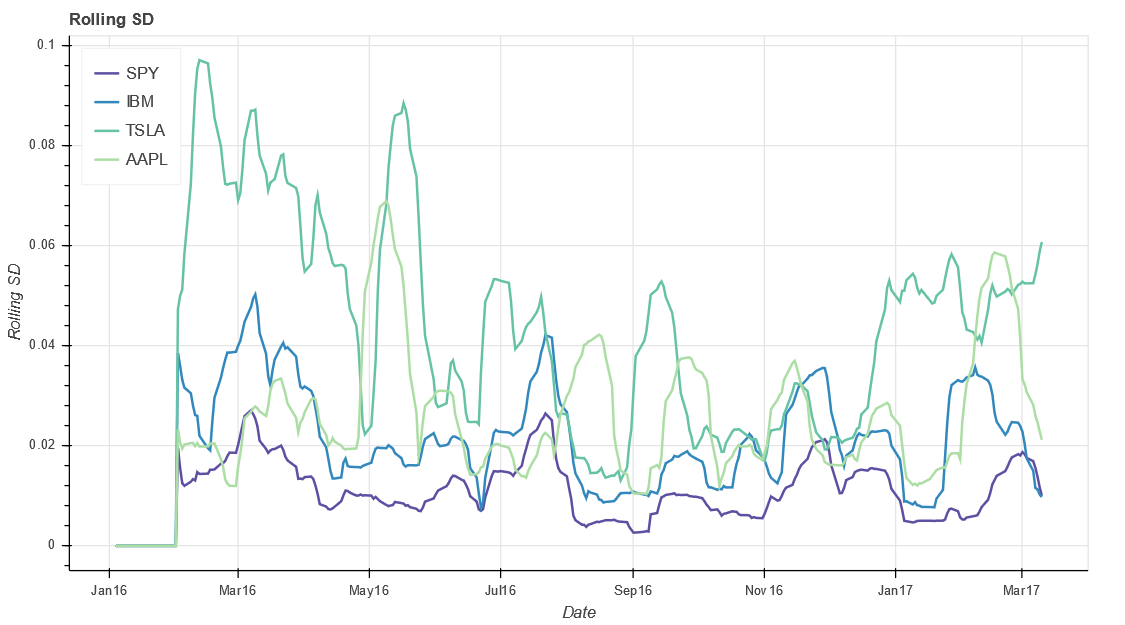
\includegraphics[height=0.4\textheight,width=\textwidth]{rolling_sd.png}
\caption{Rolling standard deviation ($\sigma$) for the symbols IBM, TSLA and AAPL}
\label{fig:std}
\end{center}
\end{figure}

\item \underline{Momentum} is defined as:

\begin{equation}
 \label{eq:mtm}
r(t)=\frac{p(t)}{p(t-N)}-1
\end{equation}

where $N$ is the size of the window.
\end{enumerate}

Plots for rolling mean, rolling standard deviation and bollinger-bands are show in  Fig.~\ref{fig:rm}, \ref{fig:std}, and \ref{fig:bb} for IBM, TSLA and AAPL. For more details, refer to the application website \cite{pp}

\begin{figure}[!htbp]
\begin{center}
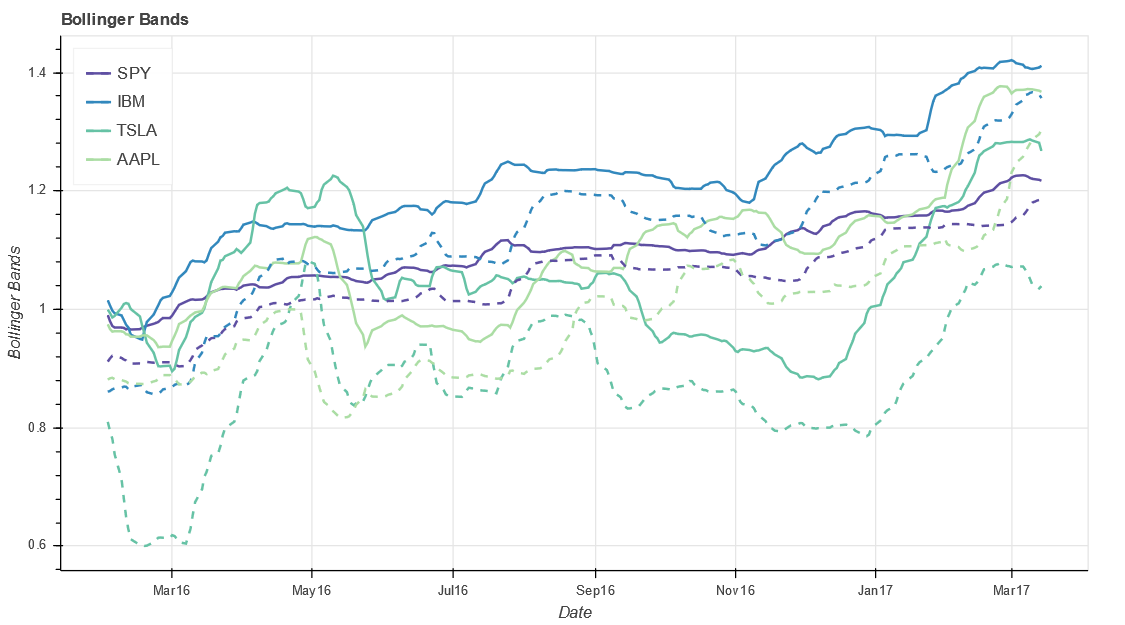
\includegraphics[height=0.5\textheight,width=\textwidth]{rolling_bb.png}
\caption{Bollinger bands IBM, TSLA and AAPL; upper are shown in solid lines and lower bands are shown in dotted lines }
\label{fig:bb}
\end{center}
\end{figure}

\section{Algorithms used in the project}
\label{sec:algos}

This section provides brief description of the algorithms used in this project.

\subsection{Convex Optimization}
\label{sec:convex}
A real-valued function defined on an interval is said to be convex if the line-segment between two points on the graph of the function lies above or on the graph. More formally, let $\mathbf{X}$ be a convex set in a real vector space and let $f: \mathbf{X}\rightarrow \mathbb{R}$ be a function, then $f$ is called \textbf{convex} if:

\begin{equation}
\label{eq:convex}
\forall x_1,x_2 \in \mathbf{X}, \forall t \in [0,1]: f(tx_1+(1-t)x_2) \leq tf(x_1)+(1-t)f(x_2 )
\end{equation}

In finance and economics, $convex$ $optimization$ plays an important role. Convex optimization algorithms are easy to solve, since they have one local minimum, which is also a global minimum. They can be solved using gradient-descent or other numerical optimizations as Sequential Least SQuare Programming (SLSQP). Fig.~\ref{fig:convex} shows an example of the convex function.

\begin{figure}[!htbp]
\begin{center}
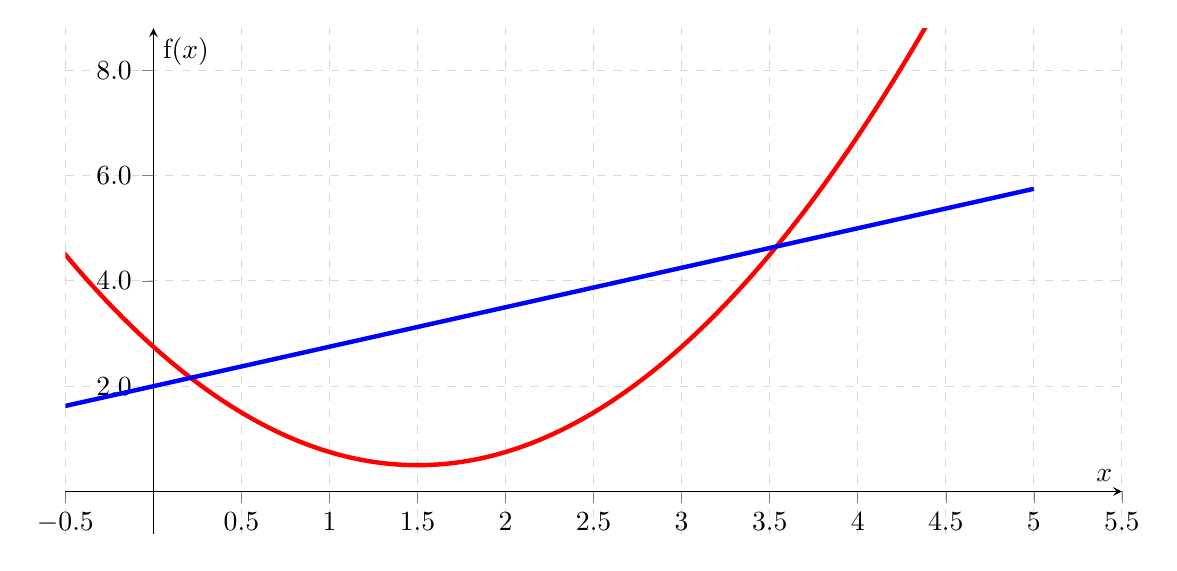
\begin{tikzpicture}
\begin{axis}[
        legend pos=north west,
        axis x line=middle,
        axis y line=middle,
        y tick label style={/pgf/number format/fixed,
                            /pgf/number format/fixed zerofill,
                            /pgf/number format/precision=1},
        grid = major,
        width=15cm,
        height=8cm,
        grid style={dashed, gray!30},
        xmin=0,     % start the diagram at this x-coordinate
        xmax= 5,     % end   the diagram at this x-coordinate
        ymin= 0,     % start the diagram at this y-coordinate
        ymax= 8,     % end   the diagram at this y-coordinate
        %axis background/.style={fill=white},
        xlabel=$x$,
        ylabel=f$(x)$ ,
        tick align=outside,
        enlargelimits=true]
      % plot the stirling-formulae
      \addplot[domain=-5:5, red, ultra thick,samples=500] {(x-1.5)^2+0.5};
       \addplot[domain=-5:5, blue, ultra thick,samples=500]{0.75*x+2};
\end{axis}
\end{tikzpicture}
\caption{Example of the convex function $f(x)=(x-1.5)^2+0.5$. The blue line describes the property of convex function in Eq.~(\ref{eq:convex})}
\label{fig:convex}
\end{center}
\end{figure}

\begin{itemize}
\item Given set of assets and time-period, find allocations of funds to assets that maximizes performance.
\item Performance metrics can be:
\begin{itemize}
\item $\max cr(t)$,
\item $\min \sigma(t)$, i.e., minimizing volatility.
\item $\max sr$
\end{itemize}
\item Framing the problem:
\begin{enumerate}
\item Provide a function $f(X)=cX+b$ to minimize.
\item Provide an initial guess for allocations.
\item Call the optimizer.
\end{enumerate}
\item Constraints: We know that allocations for each stock symbol in the portfolio should be $\leq 1$, i.e.,
\[ \Sigma_{i=0}^{k} |X_i|=1.0,
	\]
where $X_i$'s are allocations for each stock.
\end{itemize}

Below is the code snippet of the optimization in \texttt{scipy}.

\begin{tabular}{@{}|p{12.5cm}|@{}}
\hline
\begin{minted}{python}
import scipy.optimize as spo
initial_alloc=[(1.0/len(sym))]*len(sym) 
bounds=((0,1),)*len(sym) 
opt_allocs=spo.minimize(sharpe_function*-1, initial_alloc, 
	args=df, method='SLSQP',bounds=bounds,
	constraints=({'type':'eq','fun':lambda
	opt_allocs: 1-np.sum(np.abs(opt_allocs))}
	)
	); 
optimal_allocs=opt_allocs.x 
\end{minted}
\\
\hline
\end{tabular}


\vspace{0.2in}

In this project, we are trying to predict the stock- future prices values, using certain features such as  Volatility Eq.~(\ref{eq:vol}), Momentum Eq.~(\ref{eq:mtm}) and Normalized Bollinger Bands (BB) Eq.~(\ref{eq:bb_norm}). This problem will be a regression problem, as the output that we are trying to predict is a real-number. The next part of the section describes the details of the algorithms that we use in this project. Also the problem of stock prediction falls under the category of supervised learning problem, as we are given with the $y_i$ label set. In other words we trying to build a model $f$, while mapping the feature row $X_j$ to each label $y_j$, so that:

\[ f(X_j) \approx y_j \]

Regression algorithms can be of two types:
\begin{enumerate}
\item \underline{Parametric}: In this type of algorithms we use data to calculate/estimate the parameters of an equation such as $y=m\times x +c$, where $m$ is the slope of the line and $c$ is the y-intercept. Linear regression, Random-forest are examples of parametric regression algorithms.
\\
\underline{Pros and Cons}:
\begin{itemize}
\item We do not have to store the original data, so these algorithms are space efficient.
\item We cannot easily update the model as more data is gathered. We have to do complete rerun of the learning algorithm to update. Thus training usually is slow, but querying (or predicting) is fast.
\end{itemize}
\item \underline{Non-parametric}: In this type of algorithms we take the data to construct the information rather than using the predetermined model. Algorithms such as $k$-nearest neighbor is an example.
\\
\underline{Pros and Cons}:
\begin{itemize}
\item We have to store all the data points. So for huge datasets it is inefficient
\item But as the new evidence comes, the model can be easily trained. 
\end{itemize}
\end{enumerate}


\subsection{Linear regression}
\label{sec:lr}
In the simplest form the Linear regression can be expressed as :

\begin{equation}
\label{eq:lr}
f(\mathbf{X_j})=\Sigma_i\beta_i \mathbf{X_{ji}},
\end{equation}
where $\beta_j$ are the co-efficients.

\begin{figure}[!htbp]
\begin{center}
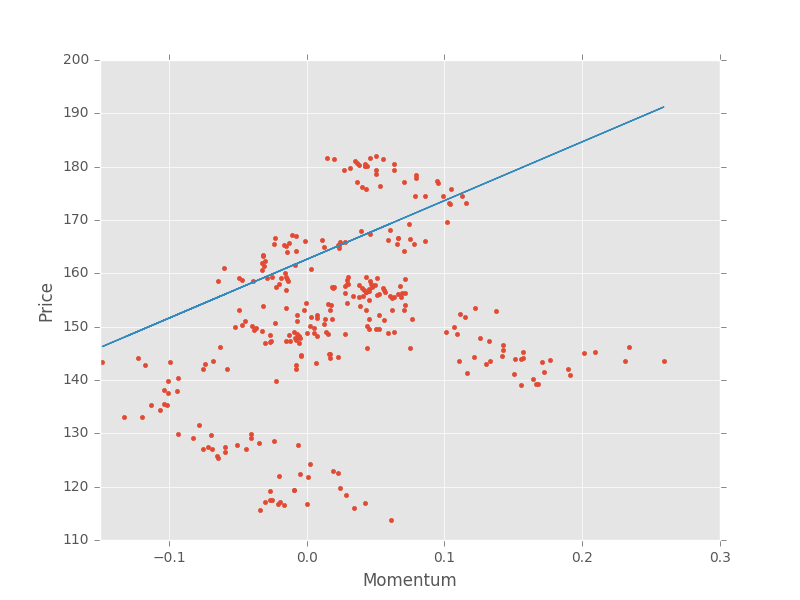
\includegraphics[height=0.4\textheight,width=\textwidth]{lr_momentum_fit.png}
\caption{Scatter plot of $y_{true}$ values vs predicted values of $y$ using linear regression for IBM stock. }
\label{fig:lr_example}
\end{center}
\end{figure}

The Figure~\ref{fig:lr_example} shows the example of linear regression fit for the IBM ticket symbol using the momentum feature. The linear fit shown in Figure~\ref{fig:lr_example} indicates that the data exhibits a lot of non-linearity and Linear regression might not give a good estimate of the  stock prediction. We will discuss the metrics used for model evaluation in Section~\ref{sec:metrics}.

\subsection{Ridge regression}
\label{sec:rr}
Ridge regression shrinks the regression coefficients by imposing a penalty on the their size \cite{ESL2}. The coefficients minimize a penalized residual sum squares.  
Ridge model solves the regression model where the loss function is the linear least-squares function and the regularization is given by the $L^2$ norm \cite{scikit-ridge}.

\subsection{Random forest regression}
\label{sec:rfr}

Random forests are ensemble (or collection) of decision trees, that output mean prediction (regression) of the individual tree for regression problems. The idea is to average many noisy but approximately unbiased models and thus reduce the variance  \cite{ESL2}.  Random-forests regressions are quite efficient especially where the data is non-linear. In the the Fig. \ref{fig:lr_example}, we have seen that the momentum is quite non-linear and thus not surprisingly, the linear-regression and so does the ridge did not work well. Figure \ref{fig:rfr_example} shows the fit for Random-forests, and this clearly indicates that predictions are clearly close enough to the true values.

\begin{figure}[!htbp]
\begin{center}
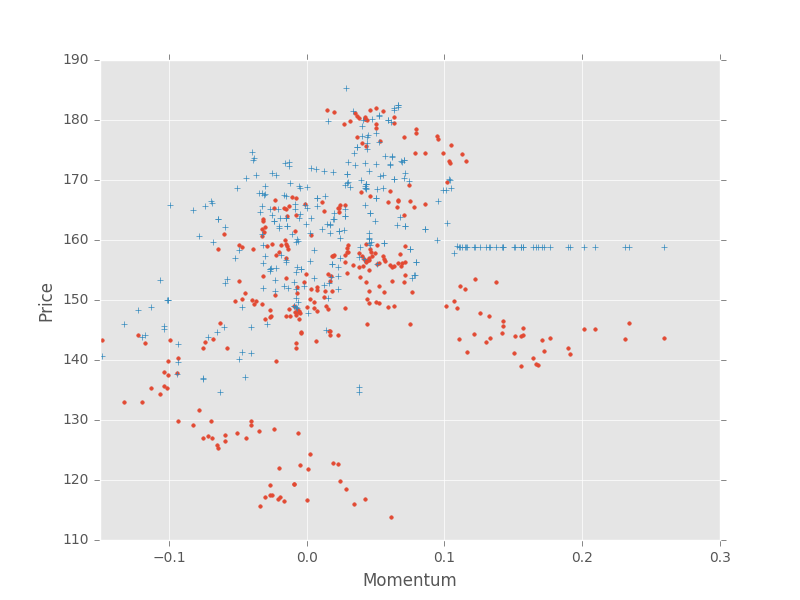
\includegraphics[height=0.4\textheight,width=\textwidth]{rfr_momentum_fit.png}
\caption{Scatter plot of $y_{true}$ values vs predicted values of $y$ using Random forest regression for IBM stock. Circles indicate true values and $+$ indicates the predicated values. }
\label{fig:rfr_example}
\end{center}
\end{figure}


\subsection{$k$-nearest neighbors (kNN)}
\label{sec:knn}

As the name implies, the prediction for a new point is based on the closest $k$-points in the training set, where closest is usually defined in terms of Euclidiean distance on the $\mathbf{p}$ dimensional feature space. As the regression problem, it take the average label of the nearest $k$-neighbors. This is a non-parametric algorithm as discussed in the earlier part of the section. From the Fig. \ref{fig:knn_example}, we see that kNN performs almost similar to Random forest regression, capturing the non-linearities in the data.

\begin{figure}[!htbp]
\begin{center}
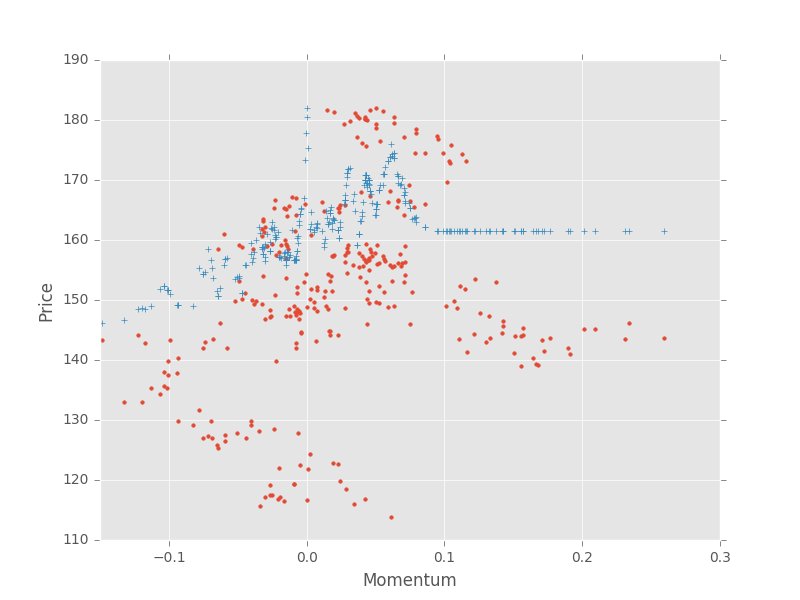
\includegraphics[height=0.4\textheight,width=\textwidth]{knn_momentum_fit.png}
\caption{Scatter plot of $y_{true}$ values vs predicted values of $y$ using $k$ nearest neighbors for IBM stock. Circles indicate true values and $+$ indicates the predicated values. }
\label{fig:knn_example}
\end{center}
\end{figure}


\subsection{Benchmark Model}
\label{sec:bench}
As a benchmark model, one could use a simple mean-model. For instance, a particular stock price can be predicted using mean of the adjusted close price. This  is the simplistic baseline model. This can be implemented using the \texttt{DummyRegressor} \cite{scikit-dummy} in \texttt{scikit-learn}.



\section{Evaluation Metrics}
\label{sec:metrics}

In the previous section, we talked about the different models that can be used for the problem of stock-price prediction. The problem of stock price prediction is not just limited to the list mentioned in Section~\ref{sec:algos}, there are many other algorithms that can be applied. But, the important question is, how can one test and compare the performance of these algorithms/models. For this problem of regression we choose two important evaluation metrics:

\begin{itemize}
\item \textbf{Root-mean-square error (RMSE)}: Mean Absolute Error (MAE), is calculated as the ratio of sum of absolute values of difference between actual value and the predicted value to number of samples. Clearly this metric indicates the average deviation of a predicted value from its actual value. This is a linear function and all errors are weighted equally.

On the other hand mean-square-error (MSE), is ratio of sum of squared deviations to the number of samples, i.e., it is the mean of the squared deviation. This is a quadratic function, and if the errors are large, they are weighted more while the small errors are weighted less (say if absolute error for a sample point is less than 1, then square of the number is much smaller). Thus in a MSE based estimator, we can clearly see how the predicted values compared to the true values. MSE would be preferred performance metric over MAE especially if you want to have a model, where large errors are particularly undesirable.  Also by taking the square-root of the MSE value we get the Standard deviation, which is again helps to predict the variability of the data. 

For this problem, minimizing the metric RMSE makes the stock price prediction accurate.
\item  \textbf{Correlation coefficient}: This metric can be used to evaluate ML algorithm is to look at the relationship between predicted value vs. actual value. Let say we have a test data, and we run our model again test data to get $Y_{predict}$, which is the stock price in this case. We can now compare the $Y_{true}$ against $Y_{predict}$. By looking at the relationship between  $Y_{true}$ and $Y_{predict}$ we say if the model is correctly predicting the values. This metric is the correction function $\rho$ and it ranges between $-1 \leq \rho \leq +1$. If $\rho=1$, then they are strongly correlated; if $\rho=-1$ they are negatively correlated and if $\rho=0$, they are not correlated. 
\end{itemize}


\section{Methodology}
\label{sec:method}
Financial stock, commodity stock come in the category of time-series data. Usually time-series data has characteristics such as drift, seasonality and stationarity associated with it. We will talk briefly these set of characteristics:

\begin{enumerate}
\item \textbf{Drift}: Prices of commodity stocks such as oil, gas, gold, etc., tend to inflate as the time progresses. Usually we see and exponential fit for such data. This property is called drift and price can be mathematically represented as:

\begin{equation}
\label{eqn:drift}
X_t=e^{\mu t}
\end{equation}

We can use  $\log$ of the above equation as:
\begin{equation}
\label{eqn:drift2}
X_t=\mu  t+\epsilon
\end{equation}

\item \textbf{Seasonality}: Time-series data can posses seasonal component, such as temperature data, where temperature increases in summer and decreases in winter. There is certain periodicity associated with the data. Such data can be represented using Fourier series.

\begin{equation}
\label{eqn:season}
X_t=\alpha\sin(\omega t) + \beta\cos(\omega t)
\end{equation}

\item \textbf{Stationarity}: This means the the distribution of $X_t$ is independent of time.

\end{enumerate}

These characteristics of the time-series data may not be particularly relevant for the financial stock, but they can be applied for the commodity stock (which is the future extension of this work).

Another important concern for the time-series is whether it is predictable. We generally assume that financial data is ergodic in nature (i.e., there is a non-zero probability that state will recur). In these time-series data we generate features with lagged data. For instance, we generate the features described in Eq.~(\ref{eq:bb_norm}), (\ref{eq:vol}), and (\ref{eq:mtm}) for a particular stock-price  with a lag of say 5 days. 

After we generate the feature data, we then split the data into $train$ and $cross$-$validation$ set. Time-series again has a very different way of generating cross-validation set.  The next section describes the cross-validation methodology in the time-series data.

\subsection{Cross-validation of time-series data}
\label{sec:crossval}
In time-series we are trying to predict the value in future. Thus the validation data has to occur \textbf{after} the training data. We just cannot pick data point at random, because there might be seasonal effects. Also we cannot have our testing set occur before the training set.

The Fig.~\ref{fig:ts_xval} shows the general two methods of handling the time-series cross validation data. The module \texttt{TimeSeriesSplit} in \texttt{sklearn} creates cross-validation sets using Forward chaining method in Fig.~\ref{fig:ts_xval}.

\begin{figure}[!htbp]
\begin{center}
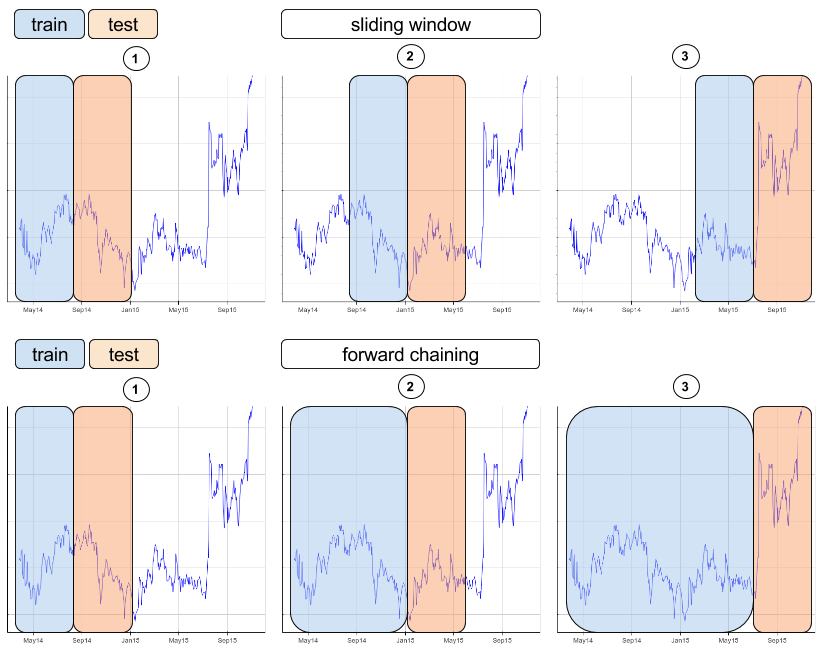
\includegraphics[height=0.4\textheight,width=\textwidth]{ts_xval.png}
\caption{Sliding window Vs. Forward chaining method}
\label{fig:ts_xval}
\end{center}
\end{figure}

\subsection{Tuning of hyperparameters}
\label{sec:hyper}
Another important aspect of the machine learning algorithms is tuning of hyper-parameters. Every algorithm has certain set of input arguments (or parameters) that needs to be tuned in order to improve the performance of the model. In the regression problem, we choose to minimize the mean-square error (Section~\ref{sec:metrics}). The mimimum value of MSE can be achieved cross-validating and carefully tuning the parameters of the regressor. The optimal parameter (or the best estimator) can be obtained using \texttt{GridSearchCV} \cite{grid} module in \texttt{sklearn}. In this section we describe the performance of the machine-learning algorithm for different values hyper-parameters.

\subsubsection{$k$-nearest neighbors}
In kNN algorithm, the important parameter that needs to be tuned is number of nearest neighbors that we want to choose in the algorithm. We cannot fix number of nearest neighbors, as it can change depending of the what stock (or ticker symbol) we choose. For instance IBM ticker symbol may give minimum MSE at different number of neighbors than TSLA (Tesla). So, instead of hard coding the regressor with the number of neighbors, we use \texttt{GridSearchCV} with parameter grid, so that regressor picks an optimal hyper-parameter for any given ticker symbol. The Fig.~\ref{fig:knn_hyper} shows the optimal value of the nearest neighbor (i.e., when the MSE is at its minimum value). The MSE plotted in the Fig.~\ref{fig:knn_hyper} is the mean MSE for all the cross-validation sets. In this and subsequent examples we have chosen 5 cross-validation folds (\texttt{TimeSeriesSplit(n\_splits=5)}).

\begin{figure}[!htbp]
\begin{center}
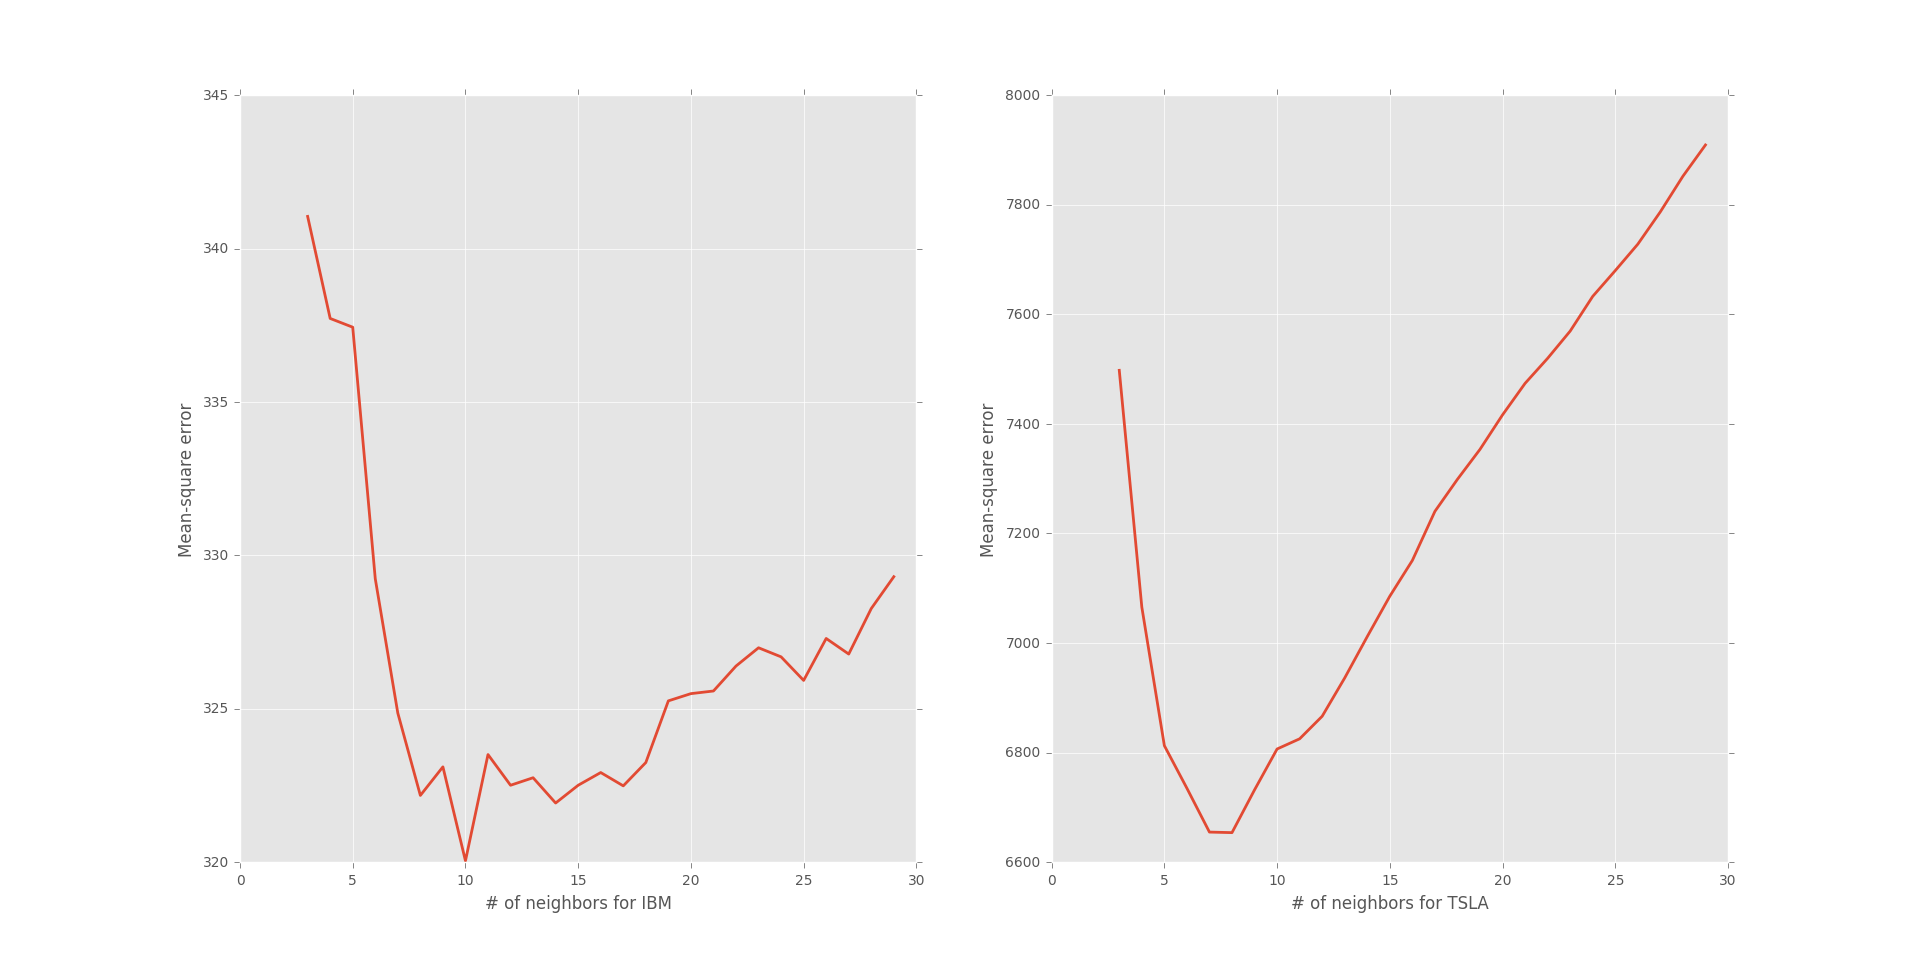
\includegraphics[height=0.4\textheight,width=\textwidth]{knn_mse_neighbors_IBM_TSLA.png}
\caption{For IBM stock the minimum value of the MSE occurs at 10 while for TSLA it occurs at $\approx$ 6}
\label{fig:knn_hyper}
\end{center}
\end{figure}

\subsubsection{Random forest regressor}
\label{sec:hyper_rfr}
In Random forest regressor, the parameter that can be tuned to improve the performance of the algorithm is number of trees or number of estimators \texttt{n\_estimators}. The Fig.~\ref{fig:rfr_hyper} shows the variation of MSE as the number of estimators is changed in the model.

\begin{figure}[!htbp]
\begin{center}
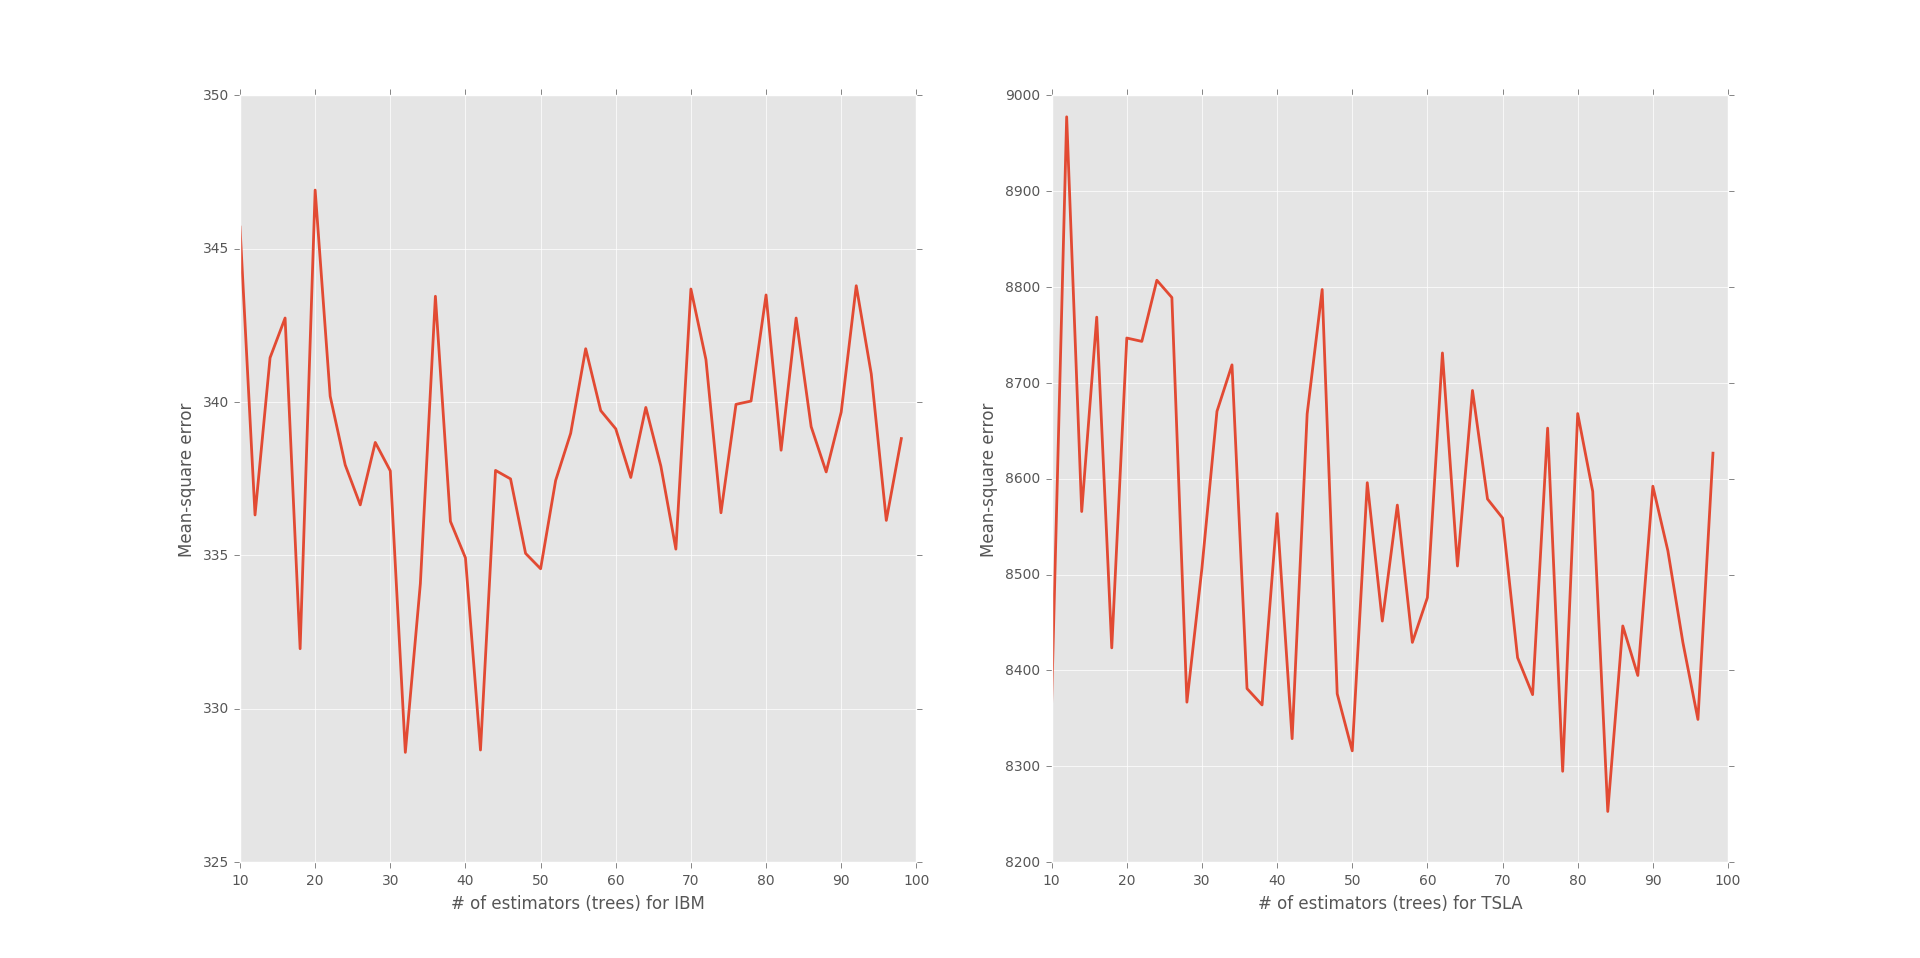
\includegraphics[height=0.4\textheight,width=\textwidth]{rfr_mse_estimators_IBM_TSLA.png}
\caption{For IBM stock the minimum value of the MSE occurs at 32, while for TSLA it occurs at 84 estimators}
\label{fig:rfr_hyper}
\end{center}
\end{figure}

\subsubsection{Ridge regression}
\label{sec:hyper_rr}
In Ridge regression, the parameter that needs to be tuned is the regularization term $\alpha$. We have considered $\alpha$ in the range of $10^{-4} \leq \alpha \leq 1$. The Fig.~\ref{fig:ridge_hyper}, shows the variation of MSE with respect to $\alpha$. The regularization term is varied using the $\log$-scale, \texttt{np.logspace(-4., 0, 20)}.


\begin{figure}[!htbp]
\begin{center}
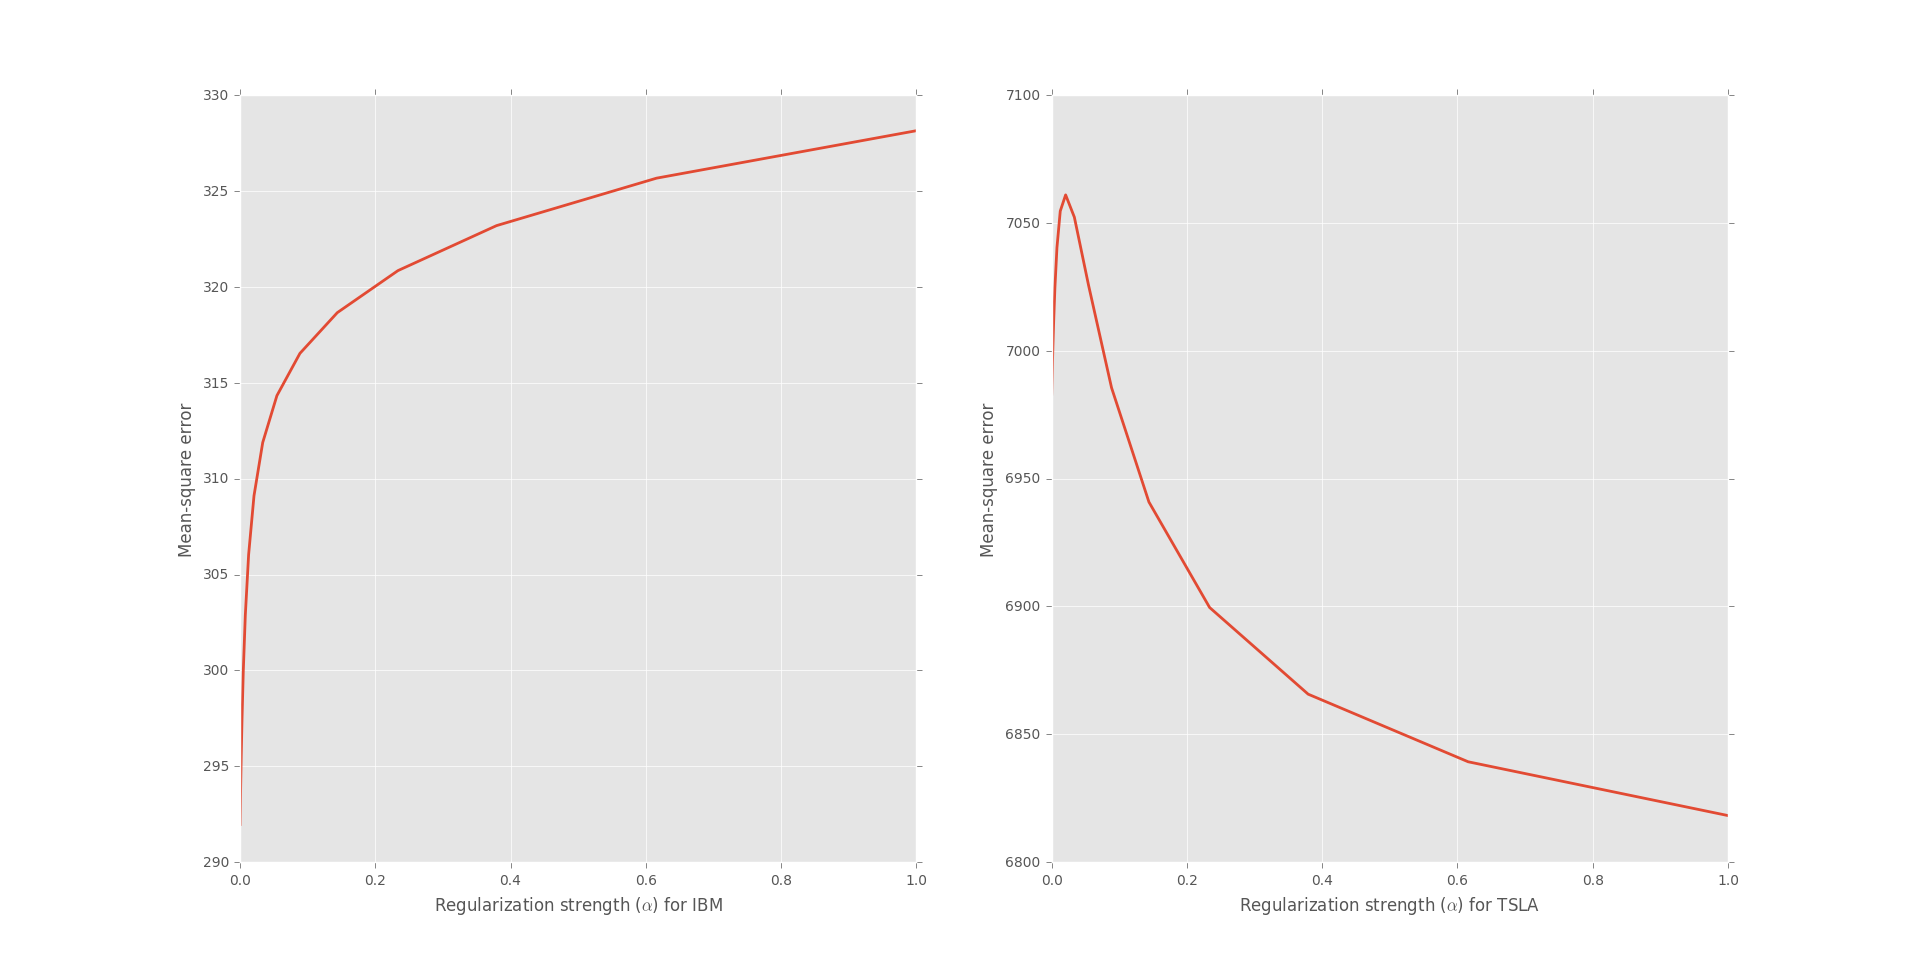
\includegraphics[height=0.4\textheight,width=\textwidth]{ridge_mse_alpha_IBM_TSLA.png}
\caption{For IBM stock the minimum value of the MSE occurs at $10^{-4}$, while for TSLA it occurs at 1.0 value of $\alpha$}
\label{fig:ridge_hyper}
\end{center}
\end{figure}

\section{Results}

In this section we discuss various results obtained for portfolio optimization, market simulator, and machine learning models. The first two subsections ~\ref{sec:opt} and ~\ref{sec:sim}, though not directly related to the the concepts of machine-learning. These two sections will be particularly important to make the trading strategies, based on the prediction values obtained from the machine learning models. For instance if the machine learning model forecasts with certain accuracy that the stock price is going to increase in next 5 days, then the trader can make decisions to buy and those improve the portfolio performance of the client. This will be the future extensions of this work.


\subsection{Portfolio optimization}
\label{sec:opt}

Portfolios in comparison with SP\&500 for the symbols, GOOG, AAPL, MSFT and IBM for duration between Jan 1 2013 to March 14 2017, for both unoptimized and optimized are shown in Fig. \ref{fig:unoptimized} and \ref{fig:optimized} respectively.

\begin{figure}[!htbp]
\begin{center}
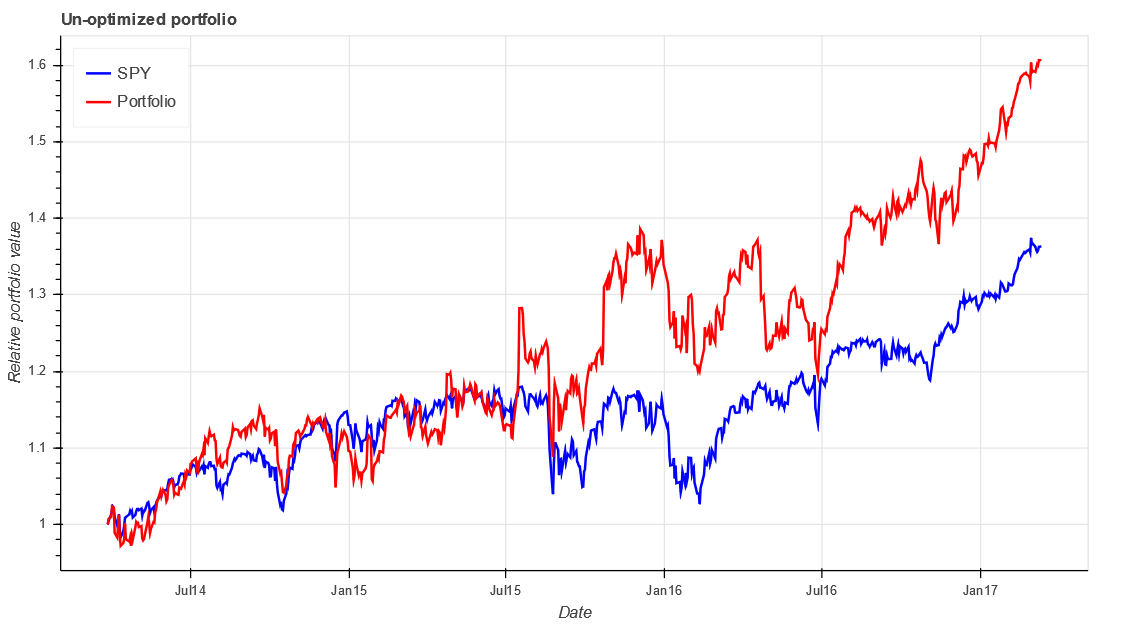
\includegraphics[height=0.5\textheight,width=\textwidth]{unoptimized.png}
\caption{Unoptimized portfolio for GOOG, AAPL, MSFT and IBM in comparison with SP\&500, with a start value of \$10000}
\label{fig:unoptimized}
\end{center}
\end{figure}

In Fig.~\ref{fig:unoptimized}, the allocations for the ticker symbols were chosen between an uniform random variables $\sim U[0,1]$, such that the sum is equals to 1. The first row in the Table~\ref{tab:alloc}, gives the random allocations. In the app  \href{http://quantfy.herokuapp.com/portfolio}{\color{blue}{http://quantfy.herokuapp.com/portfolio}} user can also pick his/her choice of the allocations. If none were chosen then the random allocations are made. From Fig.~\ref{fig:unoptimized}, we see that in the first half the graph, the portfolio is performing close S\&P500 (SPY). The parameter for unoptimized portfolio are given in Table~\ref{tab:portparam}.

\begin{table}
\begin{center}
\begin{tabular} {|c|c|c|c|c|}
\hline \hline
\textbf{Metric} & \textbf{GOOG} & \textbf{AAPL} & \textbf{MSFT} & \textbf{IBM} \\ \hline
Random allocations & 0.4682 & 0.1894 &0.2449 &0.0975 \\ \hline
Optimized allocations & 0 & 0.539 & 0.461 & 0 \\ \hline
\hline
\end{tabular}
\end{center}
\caption{Parameters computed for un-optimized and optimized portfolio}
\label{tab:alloc}
\end{table}

When we optimize the portfolio, via maximizing the Sharpe ratio, we can do a better allocation for the chosen ticker symbols.  Figure~\ref{fig:optimized} clearly improves the performance over the SPY. The optimized portfolio only allocates assets to AAPL and MSFT as given in Table~\ref{tab:alloc}. The parameters for the optimized portfolio are given in Table ~\ref{tab:portparam}. This shows an improvement in the end value over the un-optimized portfolio. Also, since we are maximizing the Sharpe ratio, we see an improvement in the value.

\begin{figure}[!htbp]
\begin{center}
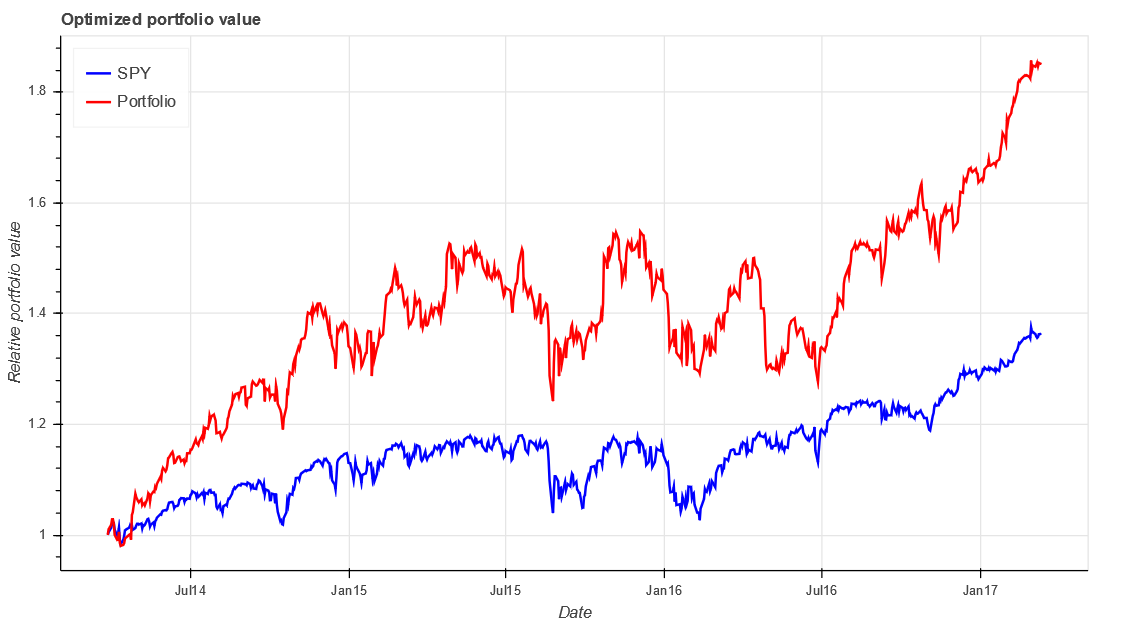
\includegraphics[height=0.5\textheight,width=\textwidth]{optimized.png}
\caption{Optimized portfolio for GOOG, AAPL, MSFT and IBM in comparison with SP\&500}
\label{fig:optimized}
\end{center}
\end{figure}


\begin{table}
\begin{center}
\begin{tabular} {|c|c|c|}
\hline \hline
\textbf{Metric} & \textbf{Un-optimized} & \textbf{Optimized}  \\ \hline
Cumulative daily return & 0.6065 & 0.8507 \\ \hline
Average daily return & 0.0007 & 0.0009\\ \hline
Standard deviation of daily return  & 0.0116 & 0.0126  \\ \hline
Sharpe ratio & 0.9624 & 1.1424 \\ \hline
End value & \$160651.061 & \$185068.0823 \\ \hline
\hline
\end{tabular}
\end{center}
\caption{Parameters computed for un-optimized and optimized portfolio}
\label{tab:portparam}
\end{table}



\subsection{Market Simulator}
\label{sec:sim}
Based on the orders file, the portfolio value can be analyzed. For instance if BUY or SELL order comes, depending on the stock price value of the order, the portfolio value changes. Using the leverage threshold, orders can be executed or fail to execute if the leverage value exceeds the threshold.

Leverage value is defined as:

\[ leverage = \frac{\Sigma|sp|} {(\Sigma(sp) + cash) }\],

where $sp$ is defined as all-stock positions \cite{GeTechCourse}. 

\begin{figure}[!htbp]
\begin{center}
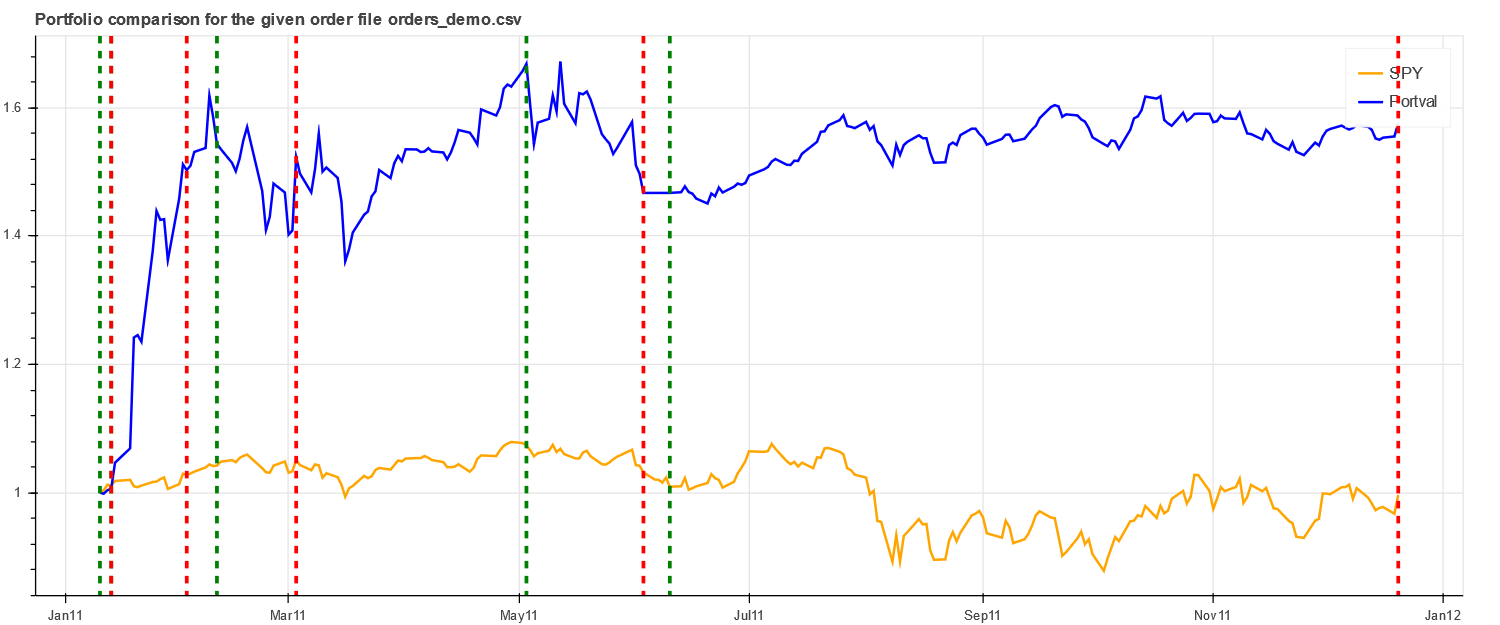
\includegraphics[height=0.5\textheight,width=\textwidth]{market.png}
\caption{Market simulator for a order file. The green vertical lines indicate a BUY order and RED vertical lines indicate a SELL order }
\end{center}
\label{fig:sim}
\end{figure}

The Fig. 9 is generated using orders file located at:
\\
\href{https://github.com/beegeesquare/QuantFy/blob/master/orders/orders_demo.csv}{\color{blue}{https://github.com/beegeesquare/QuantFy/blob/master/orders/orders\_demo.csv}}



\subsection{Machine-learning model comparison}
\label{sec:mlmodels}

Predicts the stock prices and also measures the accuracy of these forecasts. Using back-testing a method where we roll back time and measure the accuracy of these forecasts.  Slice the sample data from (historical) training set and apply the machine learning models to get the forecast.  By comparing the predictive results of the model against the historical results,  back-testing can determine whether the model has predictive value. 

The QuantFy application at: \href{http://quantfy.herokuapp.com/mlModels}{\color{blue}{http://quantfy.herokuapp.com/mlModels}}, where user can test any other ticker symbols. But for this discussion we have chosen, Google (GOOG), Apple (AAPL), Microsoft (MSFT) and IBM. These are the technology companies and the price behavior might be similar. However the code will generate a separate model for each ticker symbol.

User can select two regression algorithms from:

\begin{itemize}
\item Mean-model,
\item $k$-nearest neighbors,
\item Random forest regressors,
\item Linear regression, and
\item Ridge regression.
\end{itemize}

\begin{figure}[!htbp]

\begin{center}
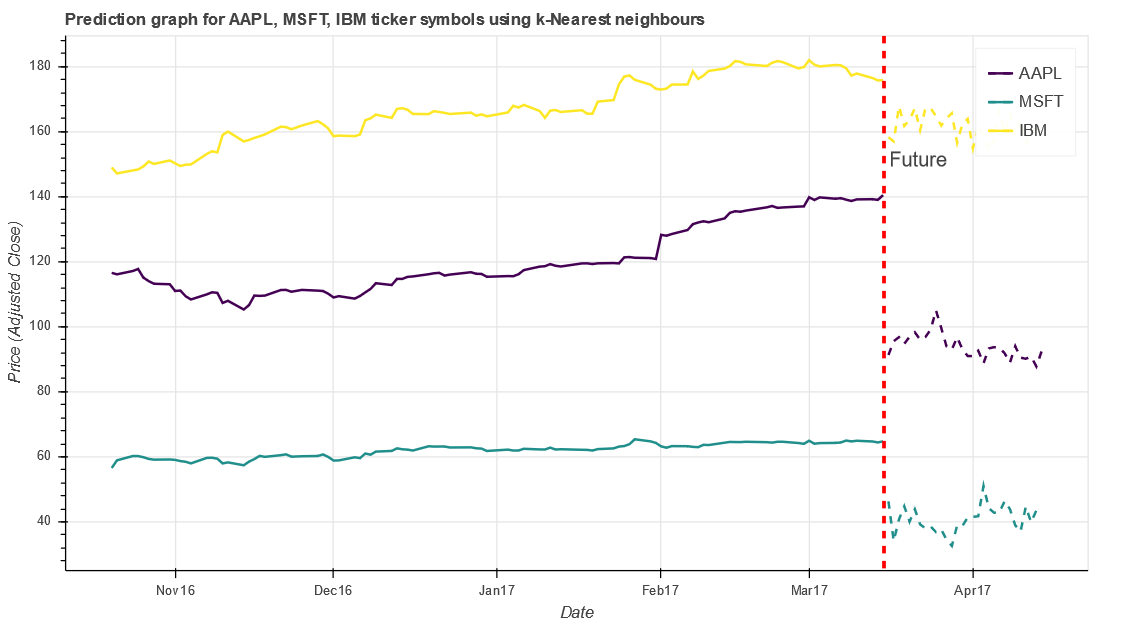
\includegraphics[height=0.4\textheight,width=\textwidth]{knn_model.png}
\caption{Prediction values for 15 days for AAPL, MSFT and, IBM using $k$-nearest neighbors }
\label{fig:knn_mdl}
\end{center}
\end{figure}

Left side of the RED dotted line indicates the past values, while the right side are the predicted values of the stock. 

\begin{figure}[!htbp]
\begin{center}
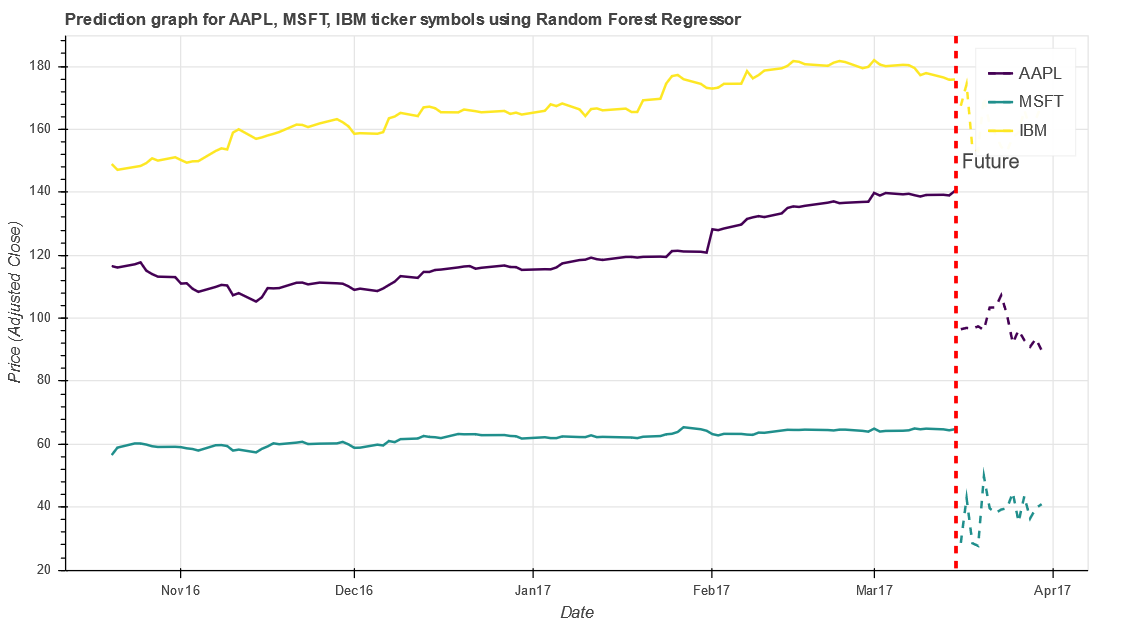
\includegraphics[height=0.4\textheight,width=\textwidth]{rfr_model.png}
\caption{Prediction values for 15 days for AAPL, MSFT and, IBM using Random forest regressor.}
\label{fig:rfr_mdl}
\end{center}
\end{figure}
\end{itemize}

Table~\ref{tab:mse} shows the Mean square error for the three ticker symbols chosen. From the Table~\ref{tab:mse} we clearly see that each ticker symbol (or stock) has different behavior. For instance AAPL stock show a linear behavior, with MSE being lower than benchmark (mean model) and showing a positive correlation coefficient for both Linear and Ridge algorithms as in Table~\ref{tab:corr}. 

Typically, as the MSE decreases the correlation-coefficient increases (close to 1). The $k$-NN seem to perform well for IBM with lowest MSE and high $\rho$.



\begin{table}
\begin{center}
\begin{tabular} {|c|c|c|c|}
\hline \hline
\textbf{ML algorithm} & \textbf{AAPL} & \textbf{MSFT} & \textbf{IBM} \\ \hline
$k$-nearest neighbors & 862.082 & 469.81 & 136.86 \\ \hline
Random forest regessor & 1390.155 & 468.274 & 164.709 \\ \hline
Linear regression &875.99 & 428.24 & 132.94  \\ \hline
Ridge regression & 876.146 & 437.069 & 132.92  \\ \hline
Mean model & 897.55 & 423.58 & 183.39  \\ \hline
\hline
\end{tabular}
\end{center}
\caption{Mean square error}
\label{tab:mse}
\end{table}

\begin{table}
\begin{center}
\begin{tabular} {|c|c|c|c|}
\hline \hline
\textbf{ML algorithm} & \textbf{AAPL} & \textbf{MSFT} & \textbf{IBM} \\ \hline
$k$-nearest neighbors &0.252 & -0.023 & 0.293 \\ \hline
Random forest regressor &  -0.33044 & -0.0761 & 0.0614  \\ \hline
Linear regression & 0.649 & -0.1706 & 0.196  \\ \hline
Ridge regression &0.677 & -0.145 & 0.197 \\ \hline
Mean model & NaN & NaN & NaN  \\ \hline
\hline
\end{tabular}
\end{center}
\caption{Correlation coefficient ($\rho$)}
\label{tab:corr}
\end{table}

However for the Microsoft (MSFT), the MSE seem to be consistently high for all the algorithms used in the project. The number of  features used in the project are less. Adding more features such as P/E ratio, volume of trades, can definitely improve the performance of the algorithm and hence correctly capture the behavior of the stock. 

We clearly see that all the algorithms used in this project provide a significant improvement over the benchmark algorithm. 

\begin{figure}[!htbp]
\begin{center}
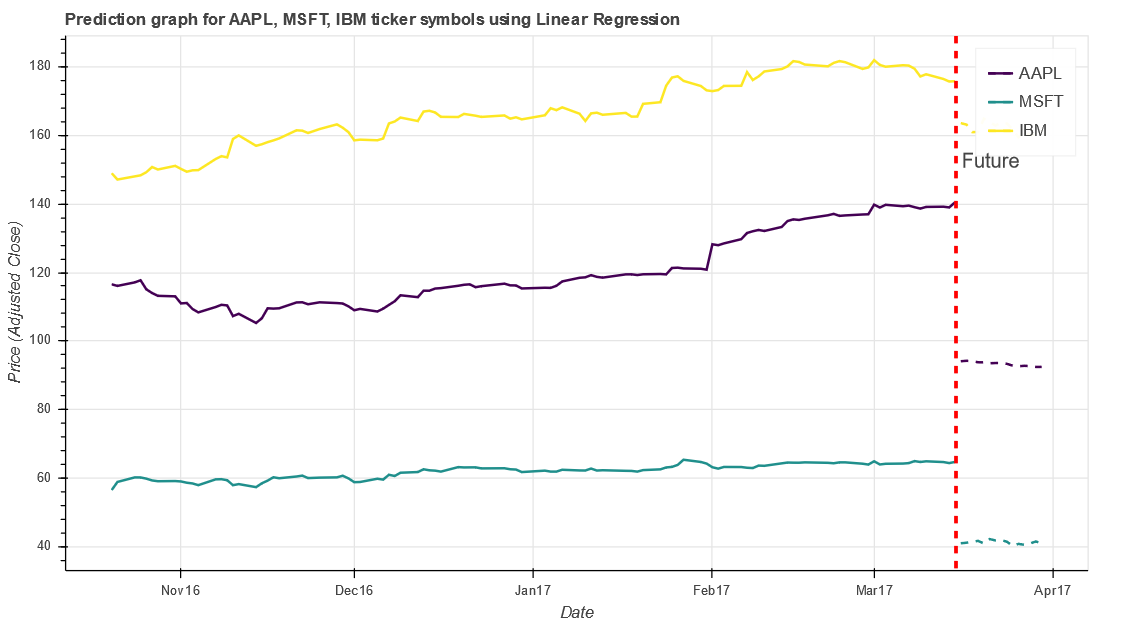
\includegraphics[height=0.4\textheight,width=\textwidth]{lr_model.png}
\caption{Prediction values for 15 days for AAPL, MSFT and, IBM using Linear regression.}
\label{fig:lr_mdl}
\end{center}
\end{figure}

\begin{figure}[!htbp]
\begin{center}
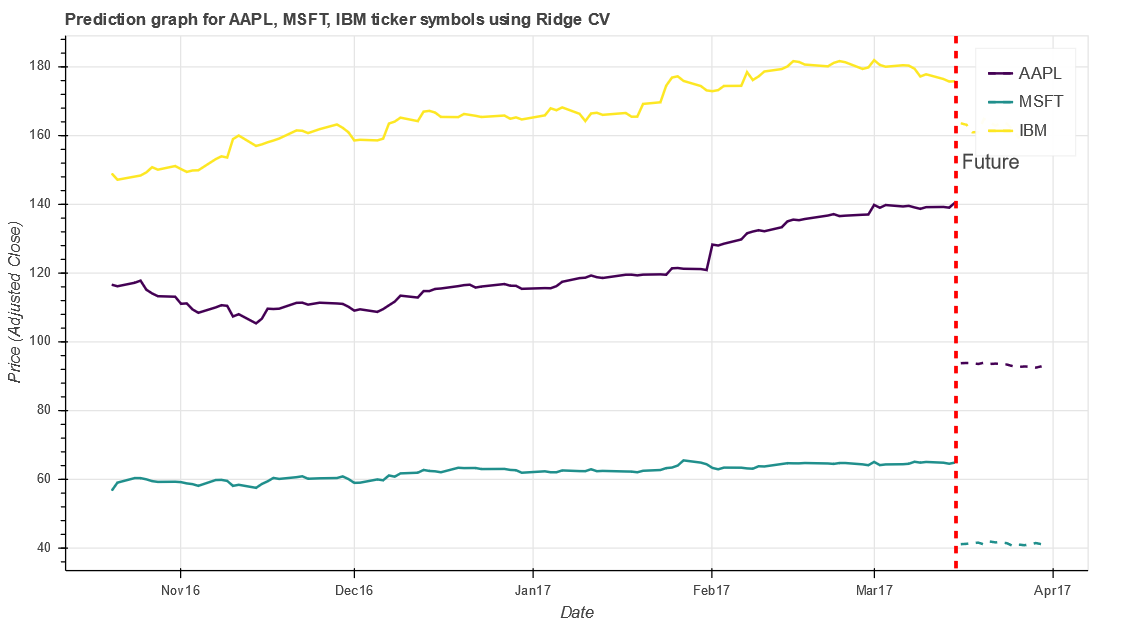
\includegraphics[height=0.4\textheight,width=\textwidth]{ridge_mdl.png}
\caption{Prediction values for 15 days for AAPL, MSFT and, IBM using Ridge regression.}
\label{fig:ridge_mdl}
\end{center}
\end{figure}


\section{Conclusion}
\label{sec:con}

This project we have provided analysis for the stock price data. Various visualizations are provided to see the behavior of particular stock price. Many parameters are computed to understand the dynamic nature of the data. Since stock price data is a time-series, we have provided the characteristics of time-series data and how it is different from any other data set.

Using convex optimization techniques, the portfolio optimization can be done and the allocations of assets to the stocks can be choose optimally.

Various machine-learning algorithms has been analyzed for the ticker symbols. We have seen that every ticker symbol has an unique behavior. For some symbols we see linear relationship and for other we see non-linear or stochastic behavior. Using the metrics such as MSE and correlation-coefficient  one can assess the quality of the prediction.

Using cross-validation and parameter tunning, we can minimize the errors, i.e., select the parameters such that the model is neither biased nor overfitted. Thus the model works well for the unseen data.

Regression algorithms possess certain drawback for the stock price predictions such as:

\begin{itemize}
\item Noisy and uncertain. 
\item It is challenging to estimate the confidence in the prediction.
\item Does not capture the stochastic behavior well.
\end{itemize}

We can overcome of these issues in regression using Reinforcement learning. As the next steps to improve the project, we will use Q-learning algorithms for the stock price predictions. Using advanced algorithms for feature selection, one can further improve the accuracy of models. 

As the further steps this application could be extended to make trading strategies based on the predictions.

Also we will extend the work for estimating the prices for commodity stocks such oil, gas, gold, etc.
\bibliography{refs}

\end{document}
